\section{What is the GPRM}

The Glasgow Parallel Reduction Machine is a virtual machine framework for multi-core programming using a task-based approach. It allows the programmer to structure their programs as a seperation of task-code (written as C++ classes) and communication code. 

Communication code is currently written in a language called GPIR which is a purely functional S-expression based language that is evaluated in parallel by default with optional sequential evaluation semantics. GPIR code controls how tasks communicate with one another and whether groups
of tasks can be evaluated sequentially or in parallel.  GPIR code is compiled down further to GPRM byte-code which is evaluated by the GPRM virtual machine.

The GPRM uses task nodes which consists of a task kernel and a task manager.

Task code is represeted as a task kernel. A task kernel is a self contained unit, typically represented as a C++ class.
To create a task kernel, the C++ class needs to be in the \textit{GPRM::Kernel::namespace}.

Communication code is represented as a task manager. A task manager "co-ordinates" communication between one or more task kernels, and
is represented as a function which can be called from a C++ program.\cite{GPRM}

\newpage

\begin{figure}[ht]
\pdfimageresolution=110
\begin{center}
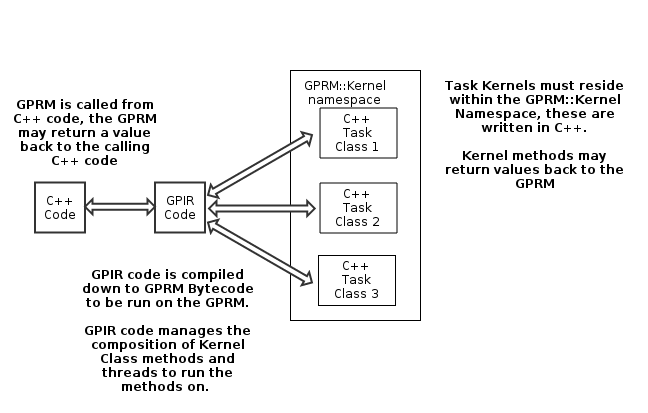
\includegraphics{graphs/gprm.png}
\caption{A simple overview of the GPRM framework}
\end{center}
\end{figure}
